\documentclass{beamer}
%\usetheme{Ilmenau}
%\usecolortheme{beaver}

\usepackage[slovak,american]{babel}
\usepackage[utf8]{inputenc}
\usepackage{graphicx}
\usepackage{adjustbox}
 \usepackage{xcolor}
 
 \newsavebox\MBox
\newcommand\Cline[2][red]{{\sbox\MBox{$#2$}%
  \rlap{\usebox\MBox}\color{#1}\rule[-2.2\dp\MBox]{\wd\MBox}{1pt}}}

%\usefonttheme{serif}

\definecolor{UKOrange}{HTML}{ef9424} %
\definecolor{UKBrown}{HTML}{a96d5e} %
\definecolor{UKLight}{HTML}{d8b6ab} %
\definecolor{UKDark}{HTML}{7a4f44}
\definecolor{UKDarker}{HTML}{4d312b} 
\definecolor{UKDarkest}{HTML}{2e1e1a}
\definecolor{UKRed}{HTML}{bf1f1c}

\setbeamertemplate{footline}[frame number]{}
\setbeamertemplate{navigation symbols}{}

%\usecolortheme{beaver}
\setbeamertemplate{itemize item}[square]
\setbeamercolor{itemize item}{fg = UKBrown}
\setbeamercolor{itemize subitem}{fg = UKLight}
\setbeamercolor{enumerate item}{fg = UKDark}

\setbeamercolor{footnote}{fg=UKLight}
\setbeamercolor{footnote mark}{fg=UKLight}
\setbeamerfont{footnote}{size=\tiny}
\renewcommand\footnoterule{}

\usetheme{default}
\beamertemplatenavigationsymbolsempty
\setbeamercolor{title}{fg=white, bg=UKBrown}
\setbeamercolor{frametitle}{fg=white, bg=UKBrown}
\setbeamercolor{block title}{bg=UKBrown, fg= white}
\setbeamercolor{block body}{bg =UKLight, fg = UKDarkest}

\useoutertheme[subsection=false]{miniframes}
\AtBeginSection[]{\subsection{}}

\setbeamercolor{below lower separation line head}{bg=UKDark}
\addtobeamertemplate{headline}{}{%
  \begin{beamercolorbox}[colsep=0.5pt]{below lower separation line head}
  \end{beamercolorbox}
}
%\setbeamercolor*{mini frame}{fg=white,bg=UKRosy}
\setbeamercolor{section in head/foot}{fg=UKLight, bg=UKDark}

%\setbeamertemplate{itemize/enumerate body begin}{\normalsize}
%\setbeamertemplate{itemize/enumerate subbody begin}{\normalsize}




%\newcommand{\codeblock}[2]{ \begin{block}{#1} \begin{verbatim}#2\end{verbatim}\end{block}}

%\defbeamertemplate*{title page}{customized}[1][]
%{
%  \begin{centering}
%    \begin{beamercolorbox}[sep=8pt,center]{title}
%      \usebeamerfont{title}\inserttitle
%    \end{beamercolorbox}
%  \end{centering}
%  \bigskip
%
%\begin{columns}[onlytextwidth,T]
%
%
%  \column{27mm}
%  \includegraphics[width=27mm]{images/logoFMFI.png}
%  
%  \column{\dimexpr\linewidth-54mm-6mm}
%  \centering
%  \vspace{5mm}  
%  \usebeamerfont{author}\insertauthor\par
%  \vspace{5mm}
%  \usebeamerfont{institute}\insertinstitute\par
%
%  \column{27mm}
%  \includegraphics[width=27mm]{images/logoUK.png}  
%\end{columns}
%\centering
%\vspace{7mm}
%  \usebeamerfont{date}\insertdate\par
%}


\title[Príznaky]{Rozpoznávanie obrazcov - 1. cvicečenie \\ Príznaky}
\author[Viktor Kocur]{Viktor Kocur \\{\small viktor.kocur@fmph.uniba.sk}}
\institute{DAI FMFI UK}
\date{17.2.2019}
%\titlegraphic{\includegraphics[width=2.7cm]{images/logoFMFI.png}\hspace*{1cm}~%
%   \includegraphics[width=2.7cm]{images/logoUK.png}
%}


\begin{document}
\selectlanguage{slovak}

\begin{frame}[plain]
  \titlepage  
\end{frame}

\section{Úvodné informácie}
%\subsection{Introduction}

\begin{frame}
\frametitle{Kontaktné informácie}

\begin{itemize}\setlength\itemsep{1em}
\item Miestnosť: I-4
\item Konzultácie: Dohodou mailom, ideálne po 13:00
\item Mail: viktor.kocur@fmph.uniba.sk, kocurvik@gmail.com
\item Stránka: \url{https://dai.fmph.uniba.sk/w?title=Course:Rozpoznavanie_obrazcov}
\item GitHub: \url{https://github.com/kocurvik/edu}
\end{itemize}

\end{frame}


\begin{frame}
\frametitle{Podmienky pripustenia ku skúške}
Za cvičenia je možné získať dohromady 40 bodov:
\vspace{1em}
\begin{itemize}\setlength\itemsep{1em}
\item 10b - Aktívna účasť na cvičeniach
\item 5b - Predbežný report k projektu
\item 25b - Projekt (prezentácia, finálny report, kód)
\end{itemize}

\vspace{1em}
Dohromady je nutné získať aspoň 20 bodov z cvičení!
\end{frame}

\begin{frame}
\frametitle{Projekt}
Dva druhy projektu:
\begin{enumerate}\setlength
\item Extrakcia príznakov + klasifikácia
\item Klasifikácia na dátach z databázy
\end{enumerate}

\vspace{1em}

Súčasťou projektu bude:
\begin{itemize}\setlength
\item Predbežný report - info o vybraných dátach a metódach
\item Prezentácia
\item Finálny report + Kód
\end{itemize}
\vspace{1em}

Termín zadania a odovzdávania sa ešte upresní!
\end{frame}

\section{Obrazce}

\begin{frame}
\frametitle{Dva popisy}

\begin{block}{Obrazec}
Obrazec (pattern) je formálny popis objektu.
\end{block}

\begin{block}{Štatistický popis}
Obrazec je vektor príznakov z príznakového priestoru napr. z $\mathbb{R}^n$.
\end{block}

\begin{block}{Syntaktický popis}
Obrazec je reťazec slov z určitého jazyka, kde tieto slová sú primitíva daného jazyka.
\end{block}

\end{frame}

\begin{frame}
\frametitle{Klasifikácia - štatistický popis}

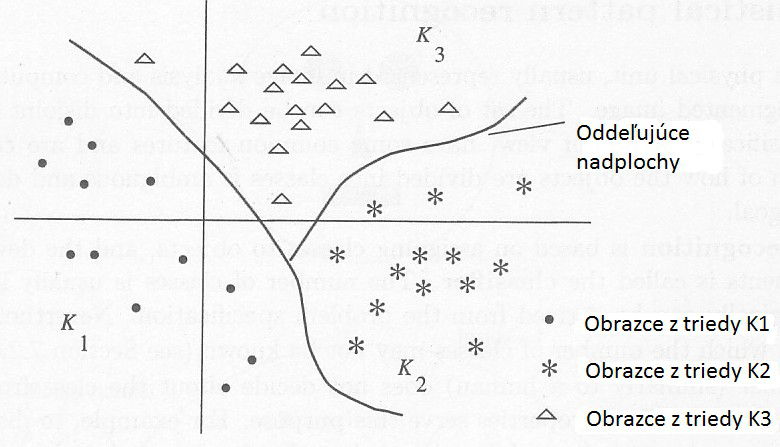
\includegraphics[width=\textwidth]{triedy.png}

\end{frame}

\begin{frame}
\frametitle{Štatistický popis - príklad}
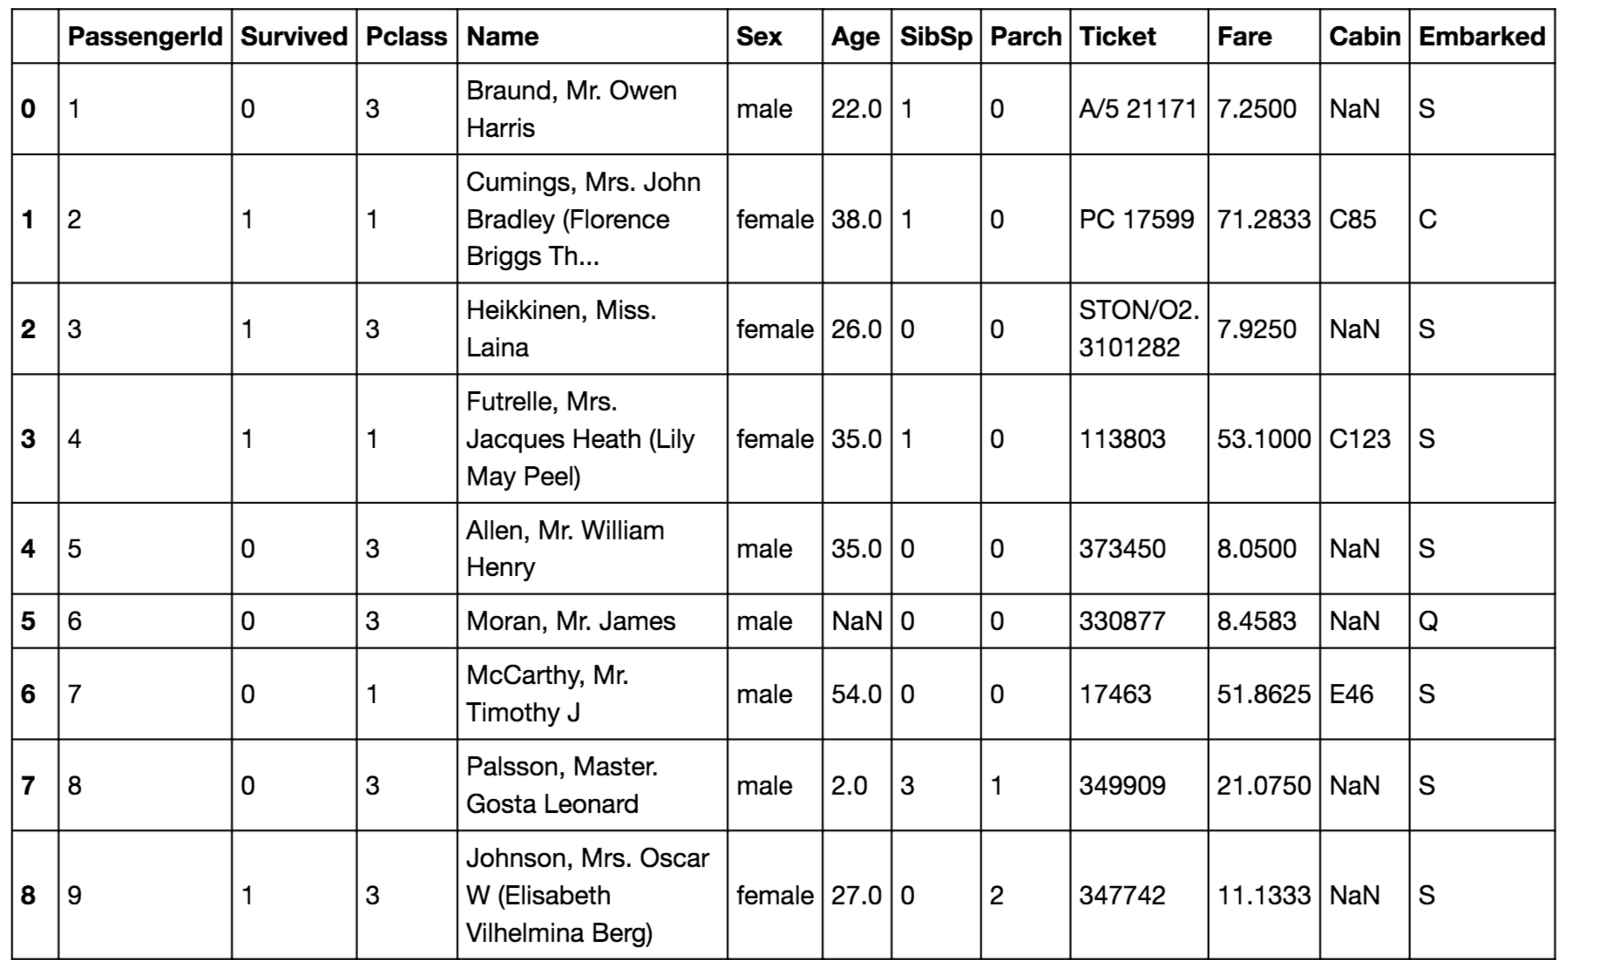
\includegraphics[width=\textwidth]{titanic.png}
\end{frame}

\section{Vizuálne príznaky}

\begin{frame}
\frametitle{Lokálne vs. globálne príznaky}
\centering
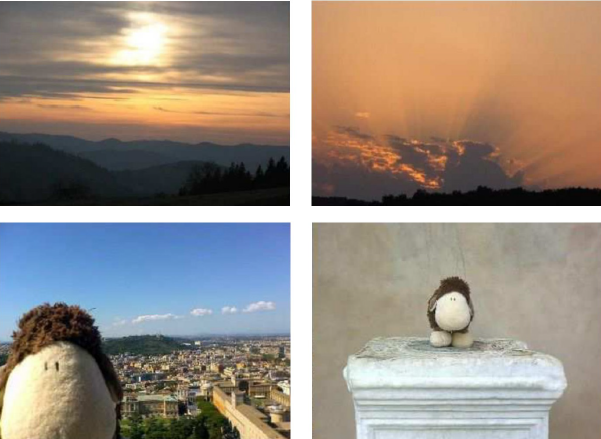
\includegraphics[width=0.8\textwidth]{locvglob.png}
\end{frame}

\begin{frame}
\frametitle{Inštancia vs. trieda}
\centering
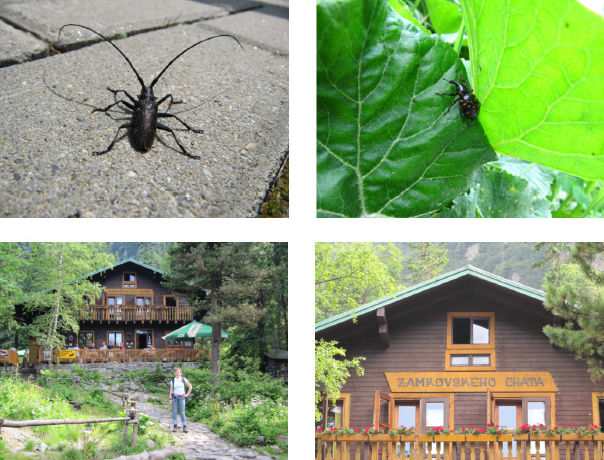
\includegraphics[width=0.8\textwidth]{instance.png}
\end{frame}

\begin{frame}
\frametitle{Tvarové príznaky}
\centering
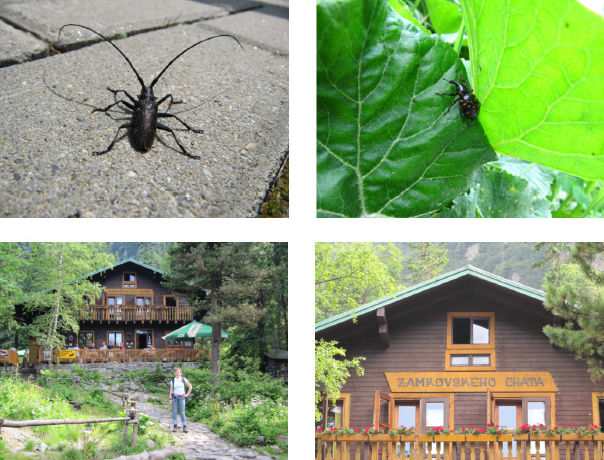
\includegraphics[width=0.8\textwidth]{instance.png}
\end{frame}

\begin{frame}
\frametitle{Farebné príznaky}
\centering
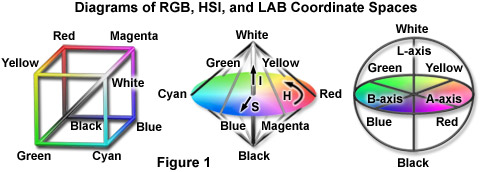
\includegraphics[width=0.8\textwidth]{colorspaces.jpg}
\end{frame}

\begin{frame}
\frametitle{Textúry}
\centering
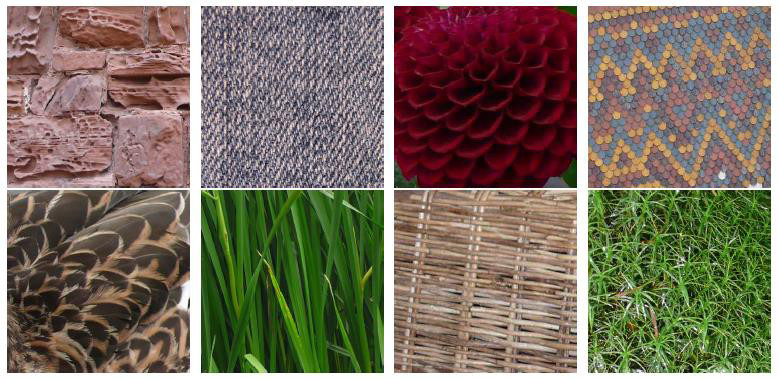
\includegraphics[width=\textwidth]{textury1.png}
\end{frame}

\begin{frame}
\frametitle{Introduction}

  \begin{columns}[onlytextwidth,T]
      \column{30mm}
      \centering
      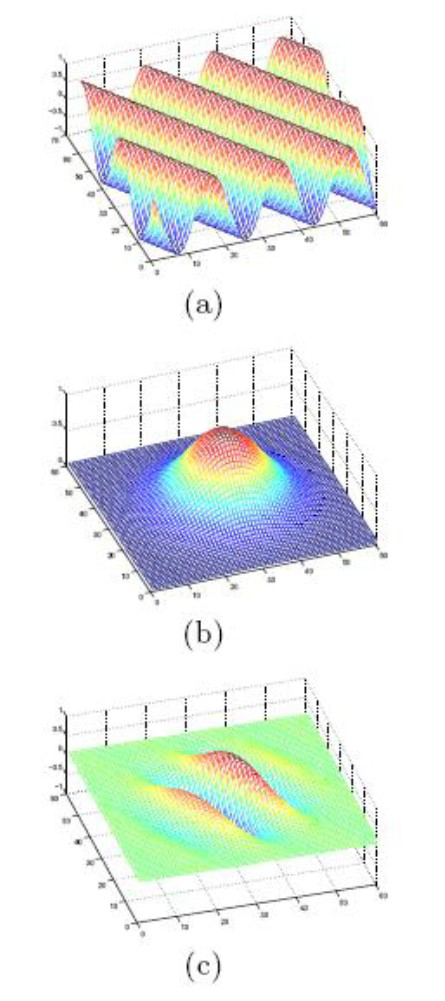
\includegraphics[width=30mm]{gabor1.png}


      \column{80mm}
      \centering
      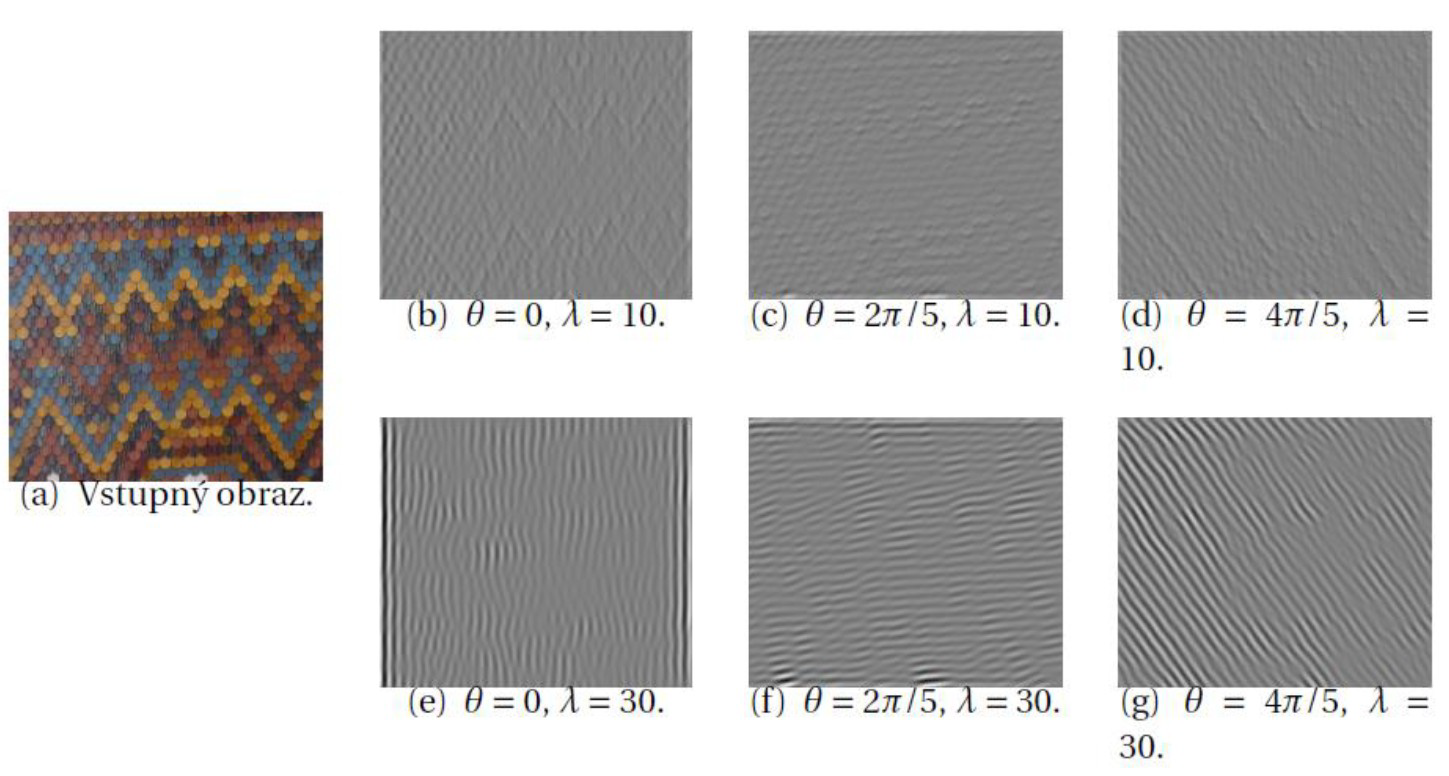
\includegraphics[width=80mm]{gabor2.png}
  \end{columns}
\end{frame}

\begin{frame}
\frametitle{Rohy, Bloby, HOG}
\centering
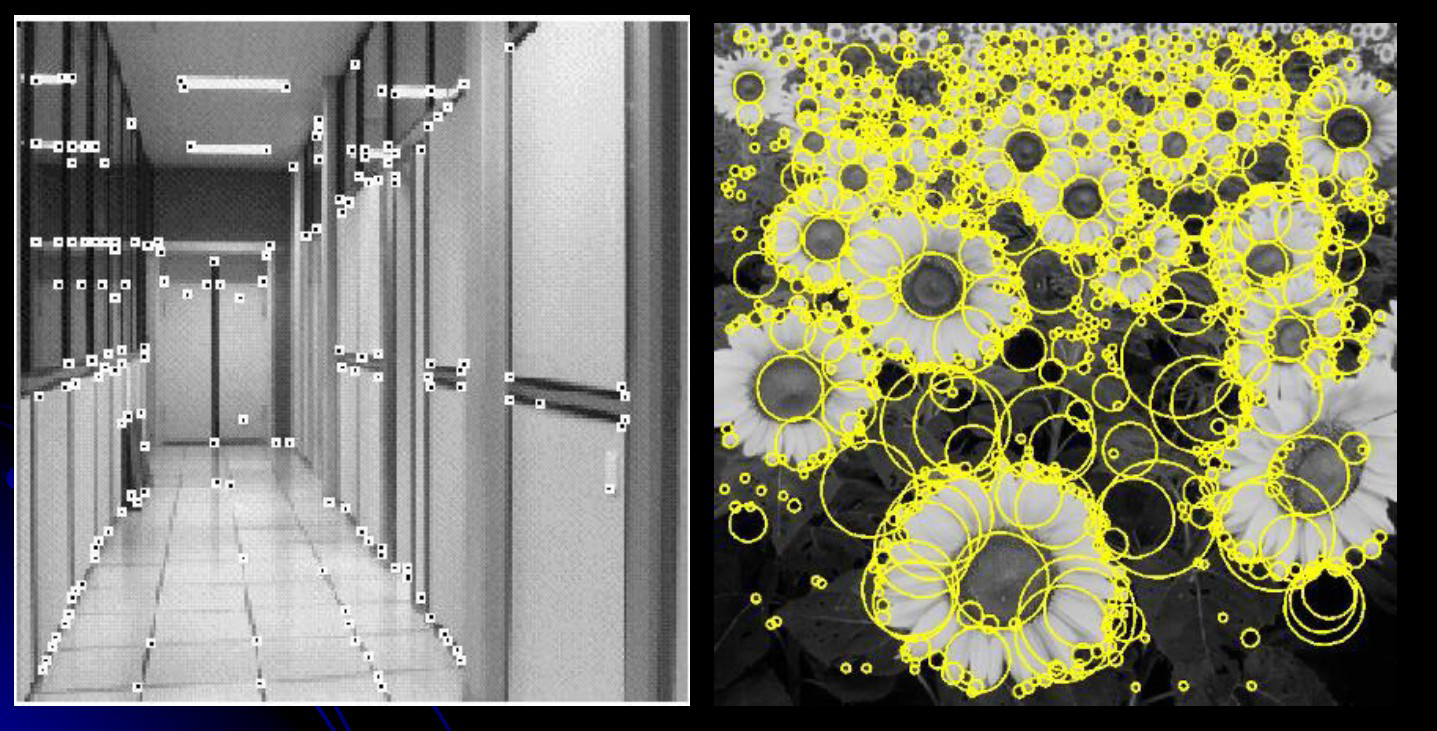
\includegraphics[width=0.6\textwidth]{local1.png}\\
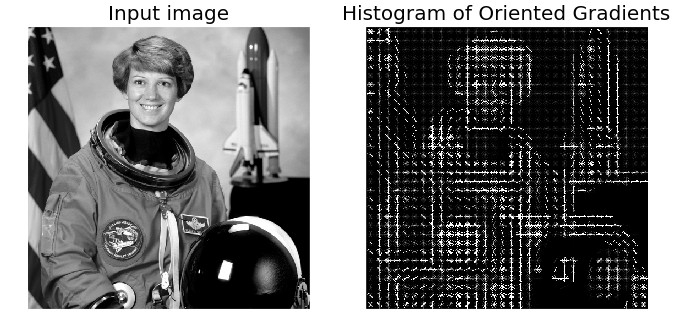
\includegraphics[width=0.7\textwidth]{local2.png}
\end{frame}

\begin{frame}
\frametitle{Úloha}
      \centering
      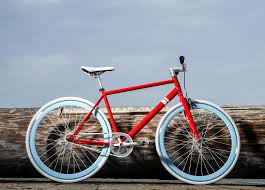
\includegraphics[width=45mm]{bike.png}
      
      \vspace{1em}

  \begin{columns}[onlytextwidth,T]
      \column{50mm}
      \centering
      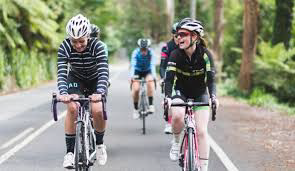
\includegraphics[width=45mm]{bike2.png}

      \column{50mm}
      \centering
      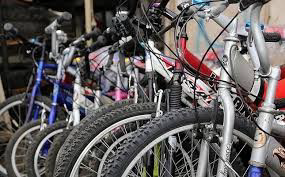
\includegraphics[width=45mm]{bike3.png}
        \end{columns}
\end{frame}

\begin{frame}
\frametitle{Úloha}
\centering

\includegraphics[width=0.8\textwidth]{bike4.png}
\end{frame}


\begin{frame}
\frametitle{Úloha}
      \centering
      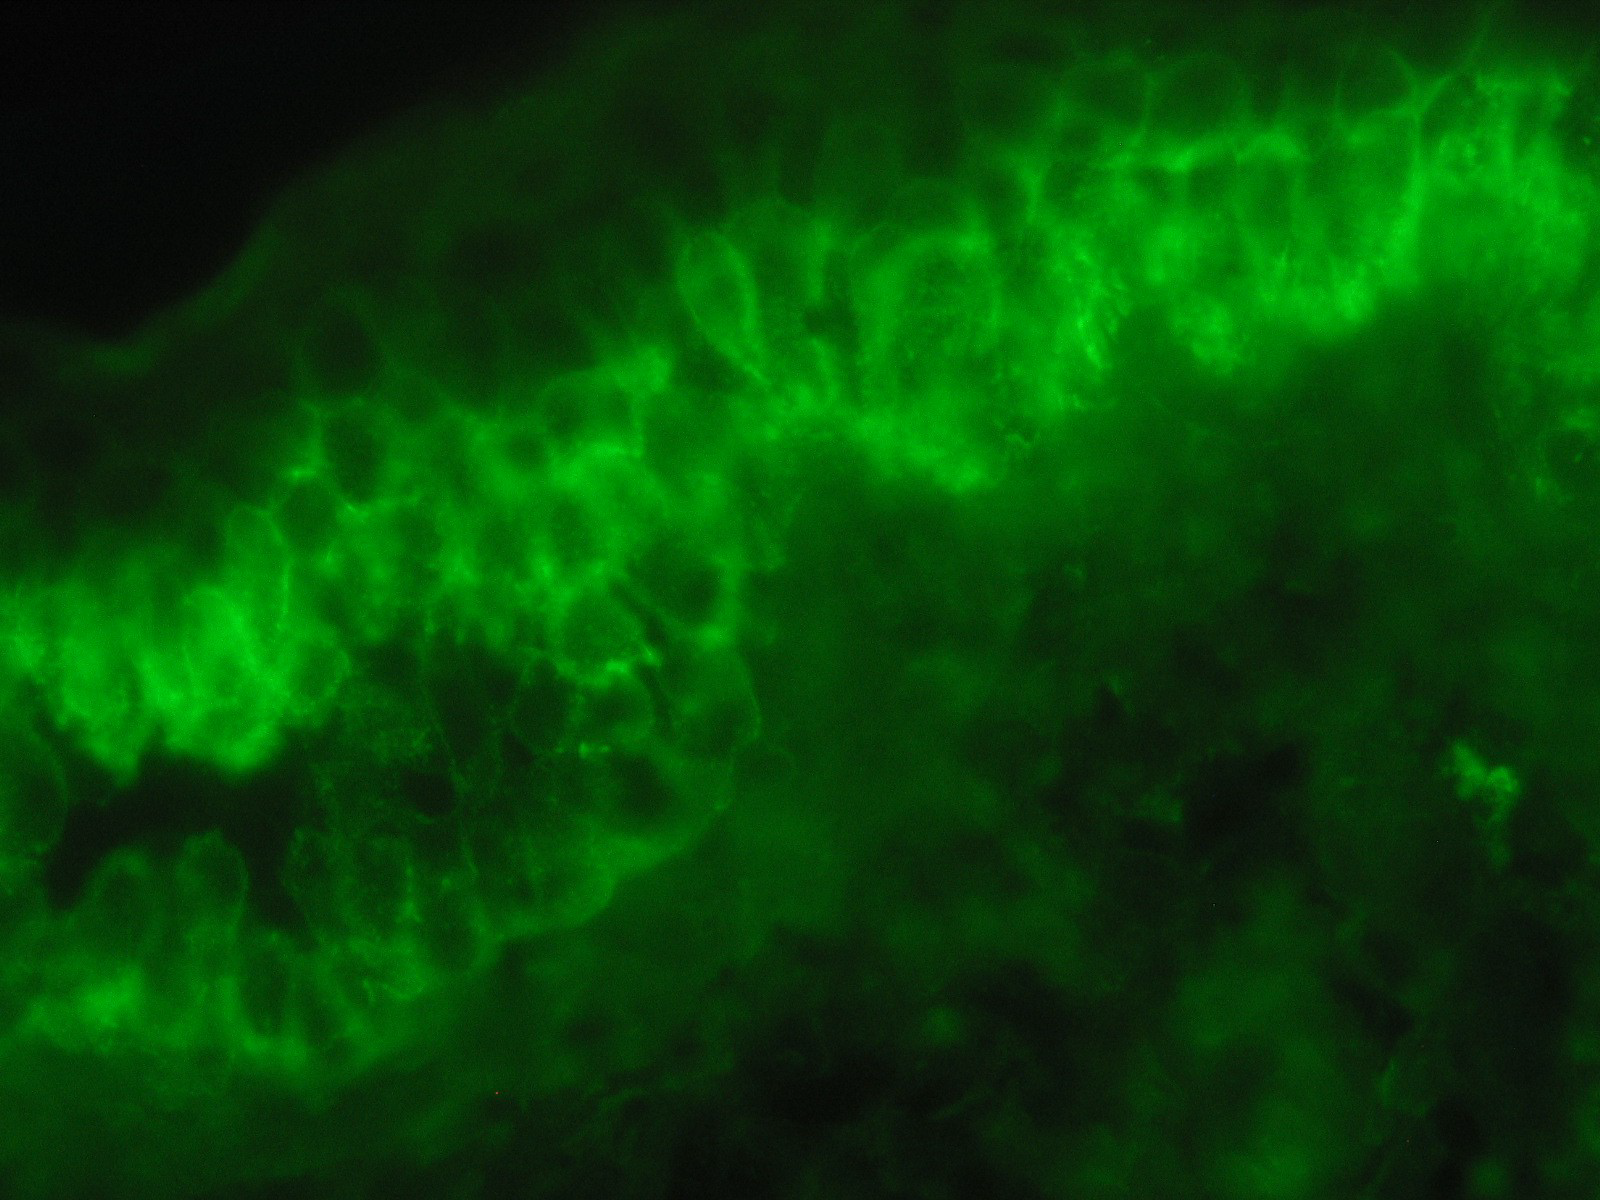
\includegraphics[width=45mm]{cell1.png}
      
      \vspace{1em}

  \begin{columns}[onlytextwidth,T]
      \column{50mm}
      \centering
      \includegraphics[width=45mm]{cell2.png}

      \column{50mm}
      \centering
      \includegraphics[width=45mm]{cell3.png}
        \end{columns}
\end{frame}

\begin{frame}
\frametitle{Úloha}

  \begin{columns}[onlytextwidth,T]
      \column{55mm}
      \centering
      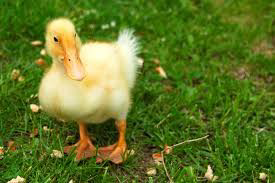
\includegraphics[width=50mm]{duck1.png}

      \column{55mm}
      \centering
      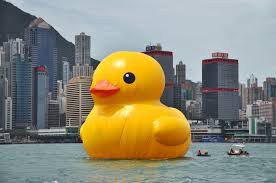
\includegraphics[width=50mm]{duck2.png}
        \end{columns}
\end{frame}

\begin{frame}
\frametitle{Úloha}
\centering
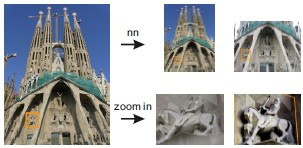
\includegraphics[width=\textwidth]{sagrada.png}
\end{frame}




\end{document}